\RequirePackage{silence}
\WarningFilter{latexfont}{Font shape}
\WarningFilter{latexfont}{Some font shapes were not available}
\documentclass[conference, onecolumn]{IEEEtran}

\usepackage{iftex}
\usepackage{geometry}
\geometry{left=4cm, right=4cm, top=2.5cm, bottom=2.5cm}
\usepackage{microtype}
\ifPDFTeX
\usepackage[utf8]{inputenc}
\newcommand{\laofont}{}
\newcommand{\tablelaofont}{}
\else
\usepackage{fontspec}
% Using Saysettha OT for all Lao text since it is provided in the project
\newfontfamily\laofont[
  Path = ../fonts/,
  UprightFont = saysettha_ot.ttf
]{Saysettha OT}
\newfontfamily\tablelaofont[
  Path = ../fonts/,
  UprightFont = saysettha_ot.ttf
]{Saysettha OT}
\fi
\usepackage{cite}
\usepackage{amsmath,amssymb,amsfonts}
\usepackage{booktabs}
\usepackage{float}
\usepackage{algorithm}
\usepackage{algpseudocode}
\usepackage{titlesec}
\usepackage{graphicx}
\usepackage[table]{xcolor}
\usepackage{svg}
\ifwindows
\svgsetup{
  inkscapeexe={"C:/Program Files/Inkscape/bin/inkscape.exe"},
  inkscapeversion=1
}
\else
\svgsetup{
  inkscapeexe={"/usr/bin/inkscape"},
  inkscapeversion=1
}
\fi
\usepackage{tabularx}
\usepackage{textcomp}
\usepackage{multirow}
\usepackage{siunitx}
\sisetup{
  detect-weight=true,
  detect-family=true,
  table-number-alignment=center,
  table-text-alignment=center
}
\usepackage{hyperref}
\hypersetup{
    colorlinks=true,
    linkcolor=blue,
    filecolor=magenta,      
    urlcolor=cyan,
    pdftitle={LaoSA: An Approach Based on Fine-tuning PLMs for Lao Sentiment Analysis},
    pdfpagemode=FullScreen,
}
\renewcommand{\thesection}{\arabic{section}}
\renewcommand{\thesubsection}{\thesection.\arabic{subsection}}
\renewcommand{\thesubsubsection}{\thesubsection.\arabic{subsubsection}}
\makeatletter
\def\thesectiondis{\arabic{section}.}
\def\thesubsectiondis{\thesectiondis\arabic{subsection}.}
\def\thesubsubsectiondis{\thesubsectiondis\arabic{subsubsection}.}
\makeatother
\titleformat{\section}[hang]{\normalfont\large\bfseries}{\thesection}{0.6em}{}
\titlespacing*{\section}{0pt}{1.4ex plus 0.3ex minus 0.2ex}{0.8ex}

\begin{document}

\title{LaoSA: An Approach Based on Fine-tuning PLMs for Lao Sentiment Analysis}

\author{
\begin{tabular}{c}
Khamtay Kongmanh\textsuperscript{1}, Quang-Vinh Pham\textsuperscript{2}, Quang-Hung Le\textsuperscript{3*} \\[0.55em]
\textsuperscript{1} Department of Information Technology, Quy Nhon University, Gia Lai, Vietnam \\
kongmanh4551050274@st.qnu.edu.vn \\[0.45em]
\textsuperscript{2} Department of Data Science, TMA Tech Group, Gia Lai, Vietnam \\
pqvinh@tma.com.vn \\[0.45em]
\textsuperscript{3} Department of Information Technology, Quy Nhon University, Gia Lai, Vietnam \\
lequanghung@qnu.edu.vn
\end{tabular}
}
\maketitle

\begin{abstract}
Effective sentiment analysis for the Lao language is hindered by a scarcity of annotated resources and the inherent noise of real-world user feedback, which often features code-mixing and informal script patterns. This study addresses these challenges by introducing a high-quality, filtered benchmark of 25,139 Lao-language reviews collected from popular digital applications. We evaluate classical baselines, a lightweight TextCNN model trained from scratch, and several state-of-the-art Pre-trained Language Models (PLMs), including XLM-RoBERTa, mBERT, and a Lao-specific mBERT-Lao, across Full Fine-tuning, Low-Rank Adaptation (LoRA), and 3-fold cross-validation settings as applicable. Our experimental results demonstrate that XLM-RoBERTa achieves superior performance with 96.64\% accuracy and an F1-macro score of 0.9617. TextCNN also provides a strong neural baseline with 94.03\% F1-macro on the fixed split, placing it between the sparse baselines and the strongest PLM variants. We also find that while Lao-oriented pretraining provides significant benefits, LoRA offers a highly efficient performance-cost trade-off, maintaining competitive accuracy with minimal trainable parameters. Our research highlights the robustness of multilingual transfer for low-resource sentiment classification and provides a publicly available dataset and code-mixing benchmark at \url{https://github.com/KT246/LaosSA}.
\end{abstract}

\begin{IEEEkeywords}
Lao Sentiment Classification, Pre-trained Language Models, TextCNN, LoRA, Low-resource NLP.
\end{IEEEkeywords}

\section{Introduction}
\label{sec:introduction}

Sentiment analysis plays an important role in e-commerce and digital-service platforms because user reviews and ratings provide direct evidence of customer satisfaction, service quality, and product perception \cite{tan2023survey,alahmadi2025generalizing,10.1007/978-3-032-21625-0_12}. For Lao-language platforms, automatic sentiment classification could support faster and more scalable analysis of user feedback from app stores, social media, and related digital channels.

The main gap is that Lao sentiment analysis remains under-resourced in both data and tooling. Publicly available annotated corpora, standardized benchmarks, and mature NLP tools for Lao are still limited \cite{lin2022laoplm,nguyen2025semi,saengsuwan2023laonlp}. The challenge is compounded by the continuous-script nature of Lao, in which word boundaries are not explicitly marked \cite{nguyen2025semi}, and by the character of real review data, which is often short, noisy, informal, and domain-specific \cite{subramanian2025kec_tech_titans,chowdhury2025mysticciol,durairaj2025overview}. As a result, methods that work well for high-resource languages do not transfer cleanly to Lao review classification.

This limitation affects both traditional and pretrained approaches. Survey work on sentiment analysis notes that rule-based systems demand substantial manual effort, while classical machine learning models remain sensitive to feature design and labeled data availability \cite{tan2023survey,alahmadi2025generalizing}. Generic multilingual PLMs are not guaranteed to perform well either, because their pretraining may underrepresent Lao and may not align closely with Lao tokenization behavior or review-specific language \cite{lin2022laoplm}. This motivates a direct comparison between strong multilingual PLMs, a Lao-supporting PLM, a lightweight neural baseline, and sparse baselines on the same Lao app-review dataset. Our working hypothesis is that stronger multilingual transfer and Lao-oriented pretraining will outperform lightweight and sparse baselines, while parameter-efficient tuning will preserve most of the gains at a lower training cost.

In this work, we study Lao sentiment classification using reviews collected from Google Play applications that are actively used in Laos. Although the initial motivation comes from e-commerce sentiment analysis, the final dataset covers a broader Lao digital-service setting, including banking, social media, and other everyday mobile applications. The main contributions are as follows:
\begin{itemize}
\item We construct and analyze a Lao sentiment dataset from real mobile application reviews used in Laos, and we document the filtering steps that produce the final train and validation splits.
\item We benchmark three pre-trained language models, namely XLM-RoBERTa, mBERT, and mBERT-Lao, under Full Fine-tuning, LoRA, and 3-Fold Cross-Validation settings, and we compare them against a lightweight TextCNN trained from scratch together with Logistic Regression, SVM, and Decision Tree baselines.
\item We report predictive performance, error patterns, and training efficiency so that model quality and training cost can be examined together.

\end{itemize}


The remainder of this paper is organized as follows. Section~\ref{sec:related_work} reviews related work on sentiment analysis, low-resource language processing, and pre-trained language models. Section~\ref{sec:dataset} describes dataset construction and analysis, including data collection, annotation, preprocessing, and descriptive statistics. Section~\ref{sec:methodology} then formulates the task, defines the evaluation protocol, and presents the modeling framework and fine-tuning strategies. Section~\ref{sec:experiments} reports the experimental setup, results, and discussion. Finally, Section~\ref{sec:conclusion} concludes the paper and outlines future directions.

\section{Related Work}
\label{sec:related_work}

The evolution of Lao sentiment analysis has followed the broader trajectory of pre-trained language model (PLM) development and low-resource adaptation. As illustrated in Figure~\ref{fig:timeline}, the progress spans from general multilingual baselines to dedicated Lao-specific benchmarks. 

\begin{figure}[H]
\centering
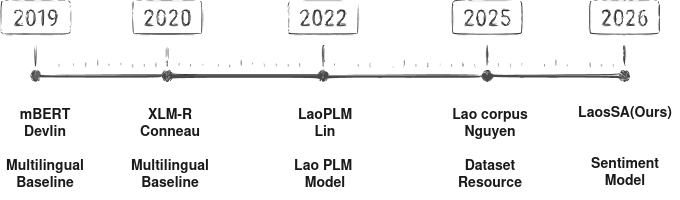
\includegraphics[width=\textwidth]{figures/LaosSA.png}
\caption{Timeline of progress toward Lao sentiment analysis, showing the evolution from multilingual baselines and monolingual pre-trained models to the current LaoSA sentiment benchmark.}
\label{fig:timeline}
\end{figure}

Early progress was marked by the introduction of multilingual BERT (mBERT) in 2019 \cite{devlin2019bert}, which provided the first massive transformer pre-training for over 100 languages, including zero-shot capabilities for low-resource scripts. However, a major limitation of mBERT remains its sub-optimal representation of Lao due to a shared vocabulary that assigns limited capacity to low-resource languages, often resulting in fragmented subword tokens for continuous scripts. This was partially addressed by XLM-RoBERTa (XLM-R) in 2020 \cite{conneau2020unsupervised}, which scaled up training data and refined cross-lingual representations. While XLM-R demonstrates significantly stronger zero-shot and few-shot performance, its primary limitation in the Lao context remains its generic pre-training objective, which does not explicitly account for the specific character boundaries or the noisy, informal code-mixing prevalent in modern digital communication.

A closely related regional example is Vietnamese e-commerce sentiment classification, where recent work reports strong results from fine-tuning PhoBERT, viBERT, and XLM-RoBERTa variants while also highlighting informal language, code-mixing, and domain-adaptation challenges that are relevant to our setting \cite{10.1007/978-3-032-21625-0_12}.

Low-resource language processing is still constrained by the lack of large corpora, annotated benchmarks, and mature preprocessing tools. For Lao, this limitation has been noted in work on word segmentation, text classification, and broader resource construction \cite{lin2022laoplm,nguyen2025semi}. Because Lao is written as a continuous script, preprocessing itself can become a source of error: tokenization and boundary detection are less straightforward than in whitespace-delimited languages \cite{nguyen2025semi}. This challenge is directly relevant to the current dataset, where many user reviews are very short and noisy.

The landscape shifted in 2022 with the introduction of LaoPLM \cite{lin2022laoplm}, the first dedicated Lao-specific pre-trained model. Its strength lies in its ability to outperform generic multilingual models on formal Lao text classification by leveraging monolingual pre-training. Nevertheless, the evaluations in LaoPLM were constrained by relatively small datasets and formal registers, leaving the task of analyzing noisy, colloquial mobile app reviews largely unaddressed. More recently, in 2025, efforts by Nguyen et al. \cite{nguyen2025semi} established a semi-supervised word-segmented corpus using large language models. While this work successfully expanded the dataset resources for Lao, the focus remained on categorization and resource generation rather than on the nuanced polarity shifts found in short-text sentiments.

Pre-trained language models are now the dominant backbone for text classification because they provide contextualized representations that can be adapted across tasks \cite{han2021pre,min2023recent}. For Lao, the distinction between monolingual and multilingual PLMs is particularly important \cite{lin2022laoplm}. A Lao-oriented model can better reflect local tokenization behavior and lexical patterns, whereas multilingual models benefit from broader pretraining but may devote less capacity to low-resource languages \cite{lin2022laoplm,ruder2021xtreme,han2021pre}.

Recent low-resource sentiment studies still report clear gains from transformer-based models, but they also show that performance depends on language fit, adaptation strategy, and dataset characteristics \cite{subramanian2025kec_tech_titans,chowdhury2025mysticciol,durairaj2025overview}. This is why our experiments compare XLM-RoBERTa and mBERT with mBERT-Lao, while also retaining a lightweight TextCNN and strong sparse baselines in the benchmark.

Our work (LaoSA, 2026) represents the next milestone by addressing these gaps across three dimensions: scale, domain, and adaptation strategy. Unlike prior benchmarks, LaoSA provides a large-scale (25,139 samples) filtered dataset specifically curated from mobile application reviews, capturing real-world noise and code-mixed patterns. Furthermore, we evaluate both full fine-tuning and parameter-efficient adaptation (LoRA) to establish practical deployment baselines that were previously underexplored for the Lao digital ecosystem.

\section{Dataset Construction and Analysis}
\label{sec:dataset}

This section details the construction and systematic refinement of the Lao sentiment benchmark, covering data collection from digital-service platforms, the manual annotation process, and the multi-stage filtering pipeline designed to ensure dataset quality.

\subsection{Data Collection}
\label{subsec:data_collection}

The reviews used in this study were collected from Google Play applications that are widely used in Laos. The corpus includes comments from banking apps, social media apps, and other digital-service applications rather than from a single e-commerce marketplace. This choice was practical: these applications produced enough Lao user feedback to build a usable sentiment dataset, and they reflect the short mobile reviews that a deployed Lao sentiment system would need to handle.

Each record contains two fields, namely the review text and a binary sentiment label. The final benchmark also retains short code-mixed reviews in which Lao words appear together with English interface terms such as \textit{app}, \textit{bug}, or \textit{OK}, provided that the overall sentiment remains interpretable. This choice keeps the released benchmark closer to real mobile feedback in Laos and directly corresponds to the code-mixing setting referenced in the released resources.

\subsection{Annotation Scheme}
\label{subsec:annotation_scheme}

The raw reviews were manually annotated with binary sentiment labels. Each review was assigned a single label based on its overall polarity: label 1 for positive sentiment and label 0 for negative sentiment. The annotation process focused on the dominant sentiment expressed in each review, including explicit praise, complaints, dissatisfaction, or statements about overall user experience. 

To improve label consistency, the annotation followed a simple set of practical guidelines. Reviews expressing clearly favorable opinions toward an application, service quality, or user experience were marked as positive, whereas reviews expressing frustration, malfunction, dissatisfaction, or criticism were marked as negative. During dataset refinement, noisy, invalid, or suspicious samples were revisited through the cleaning pipeline described below so that only reliable sentiment instances were retained in the final corpus.

\subsection{Graphetics and Tonogenesis in Lao}
\label{subsec:graphetics_tonogenesis}

Lao is a tonal language whose orthography is significantly more complex than whitespace-delimited scripts. The script is an abugida where vowels and tone markers are positioned around consonants in a non-linear fashion. This orthographic structure, or graphetics, poses significant challenges for sentiment analysis because the physical representation of the language does not rely on whitespace to delimit word boundaries \cite{enfield2007grammar,lew2014linguistic}. Central to Lao graphetics is the classification of consonants into three distinct groups—High, Mid, and Low—which dictate the fundamental tonal behavior of syllables. Table~\ref{tab:consonant_classes} summarizes these classes and their representative characters.

\begin{table}[H]
\centering
\caption{Consonant classes in the Lao script (Graphetics).}
\small
\renewcommand{\arraystretch}{1.3}
\begin{tabularx}{0.85\textwidth}{|l|X|}
\hline
\textbf{Class} & \textbf{Representative Consonants} \\
\hline
High & {\tablelaofont ຂ, ສ, ຖ, ຜ, ຝ, ຫ} \\
\hline
Middle & {\tablelaofont ກ, ຈ, ດ, ຕ, ບ, ປ, ຢ, ອ} \\
\hline
Low & {\tablelaofont ຄ, ງ, ຊ, ຍ, ທ, ນ, ພ, ຟ, ມ, ລ, ວ, ຮ} \\
\hline
\end{tabularx}
\label{tab:consonant_classes}
\end{table}

A second crucial graphetic feature is the non-linear placement of vowels. Unlike Latin scripts, Lao vowels can be preposed, postposed, superposed, or subposed relative to the initial consonant. This complexity, illustrated in Table~\ref{tab:vowel_placement}, often leads to encoding noise in informal text where users may input characters in visual rather than logical order.

\begin{table}[H]
\centering
\caption{Vowel placement in the Lao script (Graphetics).}
\small
\renewcommand{\arraystretch}{1.3}
\begin{tabularx}{0.85\textwidth}{|l|X|l|}
\hline
\textbf{Position} & \textbf{Examples} & \textbf{Type} \\
\hline
Preposed & {\tablelaofont ເ, ແ, ໂ, ໃ, ໄ} & Before consonant \\
\hline
Postposed & {\tablelaofont ະ, າ, ຳ} & After consonant \\
\hline
Superposed & {\tablelaofont ິ, ີ, ຶ, ື, ໍ} & Above consonant \\
\hline
Subposed & {\tablelaofont ຸ, ູ} & Below consonant \\
\hline
\end{tabularx}
\label{tab:vowel_placement}
\end{table}

Furthermore, the historical development of the Lao tone system, or tonogenesis, has resulted in a framework where the surface tone is determined by the interaction between the consonant class, syllable type (live vs. dead), and tone markers \cite{pittayaporn2009phonology}. In real-world user reviews, these linguistic features are often simplified or omitted, leading to semantic ambiguity. Table~\ref{tab:tone_rules} presents the complete tone determination rules for the Vientiane (standard) dialect, illustrating the complexity that NLP models must navigate in low-resource Lao sentiment classification.

\begin{table}[H]
\centering
\caption{Complete tone determination rules reflecting Lao tonogenesis results.}
\small
\renewcommand{\arraystretch}{1.3}
\begin{tabularx}{\textwidth}{|l|X|X|X|X|X|}
\hline
\textbf{Class} & \textbf{Live (No Mark)} & \textbf{Mai Ek ({\tablelaofont ◌່})} & \textbf{Mai Tho ({\tablelaofont ◌້})} & \textbf{Dead (Short)} & \textbf{Dead (Long)} \\
\hline
High & Rising & Low Falling & High & High & Low Falling \\
\hline
Middle & Low Rising & Mid & High Falling & High & Low Falling \\
\hline
Low & Mid & High Rising & High Falling & Mid & High Falling \\
\hline
\end{tabularx}
\label{tab:tone_rules}
\end{table}

\subsection{Data Preprocessing and Cleaning Pipeline}
\label{subsec:data_preprocessing}

Before final training, the raw reviews were cleaned and filtered in several stages. After manual labeling, we removed noisy content such as repeated characters, emojis, invalid symbols, and strings that did not form meaningful Lao text. Particular attention was paid to Lao-specific character errors, especially cases in which vowels appeared without consonants or in which character combinations were visually present but linguistically invalid.

To assess label quality more efficiently, we trained a lightweight screening model and compared its predictions with the manual annotations. Samples that repeatedly agreed with their labels were retained, whereas mismatched cases were rechecked and many were removed. This step served as a practical filter for suspicious or low-quality reviews before the final benchmark experiments.

We also used a separate 5-fold cross-validation auditing step for difficult cases during dataset cleaning. This step was part of data filtering only and is distinct from the 3-fold cross-validation used later for model evaluation. Reviews that were repeatedly misclassified across folds were treated as unstable, and many of them contained invalid Lao character patterns or meaningless text fragments. Table~\ref{tab:cleaning_errors} provides specific examples of the common script errors, lexical inconsistencies, and semantic noise identified through this systematic cleaning process, comparing noisy processed samples with their standard Lao corrections.

\begin{table}[H]
\centering
\caption{Comparison of preprocessing results between Processed Data and Standard Lao, illustrating common Lao script errors identified during cleaning.}
\small
\renewcommand{\arraystretch}{1.3}
\begin{tabularx}{\textwidth}{|p{0.24\textwidth}|X|X|X|}
\hline
\textbf{Error Description} & \textbf{Processed Data (version 1)} & \textbf{Standard Lao} & \textbf{English Content} \\
\hline
Vowel error \& missing a letter:\newline \textcolor{teal!70!black}{\textbf{(1)}} \textcolor{red!75!black}{{\tablelaofont ຢຸ}} $\rightarrow$ \textcolor{blue!70!black}{{\tablelaofont ຢູ່}}: missing long-vowel sign + tone mark & {\tablelaofont ກະດີ\textcolor{red!75!black}{ຢຸ}} \textcolor{teal!70!black}{\textbf{(1)}} & {\tablelaofont ກະດີ\textcolor{blue!70!black}{ຢູ່}} & it is good \\
\hline
Incorrect label \& character error:\newline \textcolor{teal!70!black}{\textbf{(2)}} \textcolor{red!75!black}{{\tablelaofont ບໍ}} $\rightarrow$ \textcolor{blue!70!black}{{\tablelaofont ບໍ່}}: missing tone mark; label mismatch & {\tablelaofont \textcolor{red!75!black}{ບໍ}ມີຫຍັງ} \textcolor{teal!70!black}{\textbf{(2)}} & {\tablelaofont \textcolor{blue!70!black}{ບໍ່}ມີຫຍັງ} & no problem \\
\cline{2-4}
\textcolor{teal!70!black}{\textbf{(3)}} \textcolor{red!75!black}{{\tablelaofont ໃສ່}} $\rightarrow$ \textcolor{blue!70!black}{{\tablelaofont ໃຊ້}}: wrong middle word; label mismatch & {\tablelaofont ພໍ\textcolor{red!75!black}{ໃສ່}ໄດ້} \textcolor{teal!70!black}{\textbf{(3)}} & {\tablelaofont ພໍ\textcolor{blue!70!black}{ໃຊ້}ໄດ້} & enough to use \\
\cline{2-4}
\textcolor{teal!70!black}{\textbf{(4)}} \textcolor{red!75!black}{{\tablelaofont ໃດ້}} $\rightarrow$ \textcolor{blue!70!black}{{\tablelaofont ໄດ້}}: wrong leading vowel sign; label mismatch & {\tablelaofont ຕິດຕັ້ງບໍ່\textcolor{red!75!black}{ໃດ້}} \textcolor{teal!70!black}{\textbf{(4)}} & {\tablelaofont ຕິດຕັ້ງບໍ່\textcolor{blue!70!black}{ໄດ້}} & cannot install \\
\cline{2-4}
\textcolor{teal!70!black}{\textbf{(5)}} \textcolor{red!75!black}{{\tablelaofont ໄຈ}} $\rightarrow$ \textcolor{blue!70!black}{{\tablelaofont ໃຈ}}: wrong leading vowel sign; label mismatch & {\tablelaofont ຂອບ\textcolor{red!75!black}{ໄຈ}} \textcolor{teal!70!black}{\textbf{(5)}} & {\tablelaofont ຂອບ\textcolor{blue!70!black}{ໃຈ}} & thank you \\
\hline
Has no semantic meaning:\newline \textcolor{teal!70!black}{\textbf{(6)}} no valid Lao word sequence & {\tablelaofont \textcolor{red!75!black}{ພາສາພໍ່າໄພຍາຍຈາຍ່}} \textcolor{teal!70!black}{\textbf{(6)}} & & \\
\cline{2-3}
\textcolor{teal!70!black}{\textbf{(7)}} punctuation and noise fragment & {\tablelaofont \textcolor{red!75!black}{. . ຜ. ວບໍ່.ບຜຊໃ}} \textcolor{teal!70!black}{\textbf{(7)}} & & \\
\cline{2-3}
\textcolor{teal!70!black}{\textbf{(8)}} non-word string & {\tablelaofont \textcolor{red!75!black}{ອອ່ນສສືອ}} \textcolor{teal!70!black}{\textbf{(8)}} & & \\
\cline{2-3}
\textcolor{teal!70!black}{\textbf{(9)}} non-word string & {\tablelaofont \textcolor{red!75!black}{ທາດດແພພະນ້ຳສສ}} \textcolor{teal!70!black}{\textbf{(9)}} & & \\
\hline
\end{tabularx}
\par\smallskip\footnotesize
\textbf{Note:} Red text marks the incorrect span in Processed Data, while blue text marks the corrected span in Standard Lao. Teal markers (e.g., \textcolor{teal!70!black}{\textbf{(1)}}) link error descriptions to specific occurrences in the text.
\label{tab:cleaning_errors}
\end{table}


After this filtering process, the remaining reviews formed the final dataset used for training and validation.





\subsection{Dataset Statistics}
\label{subsec:dataset_statistics}

Table~\ref{tab:train_val_stats} summarizes the final train and validation splits after cleaning and filtering. The two partitions remain closely matched in class balance and contain no missing text or labels. The reviews are short on average, with only a small number of much longer comments, which is consistent with the brief and noisy style of app-store feedback.

\begin{table}[H]
\centering
\caption{Final train and validation split statistics for the Lao review benchmark after filtering and preprocessing.}
\small
\setlength{\tabcolsep}{10pt}
\renewcommand{\arraystretch}{1.12}
\begin{tabular}{@{}p{0.54\textwidth}rr@{}}
\toprule
\textbf{Statistic} & \textbf{Train} & \textbf{Validation} \\
\midrule
Rows & 20,111 & 5,028 \\
Columns & 2 & 2 \\
Empty text & 0 & 0 \\
Empty label & 0 & 0 \\
Unique text & 20,095 & 5,028 \\
Duplicated text within split & 16 & 0 \\
\addlinespace[0.2em]
Negative reviews (Label = 0) & 6,312 (31.39\%) & 1,578 (31.38\%) \\
Positive reviews (Label = 1) & 13,799 (68.61\%) & 3,450 (68.62\%) \\
\addlinespace[0.2em]
Minimum text length (characters) & 2 & 3 \\
Average text length (characters) & 29.41 & 30.29 \\
Maximum text length (characters) & 618 & 506 \\
\addlinespace[0.2em]
Minimum word count & 1 & 1 \\
Average word count & 1.52 & 1.52 \\
Maximum word count & 66 & 77 \\
\bottomrule
\end{tabular}
\label{tab:train_val_stats}
\end{table}

\section{Methodology}
\label{sec:methodology}

This section presents the formal task definition for Lao sentiment classification, introduces the selected pre-trained language models, and describes the fine-tuning strategies and training objectives employed in our modeling framework.

\subsection{Problem Definition}
\label{sec:problem_definition}
\label{subsec:methodology_task}

We formulate Lao sentiment classification as a supervised binary text classification task over cleaned Lao reviews. Let the benchmark dataset be defined as
\begin{equation}
\mathcal{D} = \{(x_i, y_i)\}_{i=1}^{N},
\label{eq:dataset}
\end{equation}
where each review $x_i = (w_1, w_2, \ldots, w_n)$ is represented by the token sequence produced by a given tokenizer, and each label satisfies $y_i \in \{0,1\}$, with $0$ denoting negative sentiment and $1$ denoting positive sentiment. Each review receives a single sentence-level label corresponding to its dominant polarity, even when the text remains short, informal, or noisy.

The task is to learn a classifier $f_{\psi}$ that maps a Lao review to one of the two sentiment classes. For each input $x$, a model estimates a posterior distribution over the label space and predicts the dominant polarity according to
\begin{equation}
\hat{y} = f_{\psi}(x) = \arg\max_{c \in \{0,1\}} p_{\psi}(y=c \mid x),
\label{eq:prediction}
\end{equation}
where $\psi$ denotes the parameters of either a classical classifier or an adapted PLM-based classifier, and $c$ indexes the candidate sentiment class. This formulation keeps the task definition model-agnostic so that sparse baselines and PLM-based systems can be compared under the same prediction rule.

The benchmark is defined under several practical assumptions. Each review is treated as an independent sample without conversational context or user metadata. The experiments focus on document- or sentence-level polarity classification rather than aspect-level sentiment extraction, and all systems operate directly on the cleaned review text rather than on hand-crafted linguistic features. These assumptions keep the comparison centered on representation quality and adaptation strategy rather than on feature design or external metadata.

The evaluation protocol follows the final filtered split described in Section~\ref{subsec:dataset_statistics}. For the main benchmark, models are trained on 20,111 training samples and evaluated on a fixed validation set of 5,028 samples. In addition, a separate 3-fold cross-validation setting is used as a robustness check on the training partition. Performance is reported using Accuracy, Precision-macro, Recall-macro, and F1-macro, with F1-macro treated as the primary comparison metric because of the moderate class imbalance between positive and negative reviews.

\subsection{Pre-trained Language Models}
\label{subsec:methodology_plms}

We evaluate three PLMs: XLM-RoBERTa, mBERT, and mBERT-Lao. XLM-RoBERTa and mBERT serve as multilingual references for cross-lingual transfer \cite{ruder2021xtreme,han2021pre,min2023recent}, while mBERT-Lao provides a Lao-supporting alternative \cite{lin2022laoplm}. Table~\ref{tab:plm_overview} summarizes the main properties of the three models under the benchmark-facing names used throughout this paper. All PLM runs share the same preprocessing and evaluation protocol, and the LoRA setting attaches adapters to the query, key, and value projections.

\begin{table}[H]
\centering
\caption{Pre-training and architectural comparison of the PLMs used in the benchmark.}
\small
\setlength{\tabcolsep}{5pt}
\renewcommand{\arraystretch}{1.1}
\begin{tabular}{@{}>{\raggedright\arraybackslash}p{0.19\textwidth}>{\raggedright\arraybackslash}p{0.24\textwidth}>{\raggedright\arraybackslash}p{0.22\textwidth}>{\raggedright\arraybackslash}p{0.24\textwidth}@{}}
\toprule
\textbf{Aspect} & \textbf{XLM-RoBERTa} & \textbf{mBERT} & \textbf{mBERT-Lao} \\
\midrule
Language scope & Multilingual (100 languages) & Multilingual (104 languages) & Lao-supporting \\
Pre-training data & CommonCrawl multilingual corpus ($\sim$2.5 TB) & Multilingual Wikipedia corpus & Lao-oriented RoBERTa-style pretraining \\
Tokenizer & SentencePiece, $\sim$250k subwords & WordPiece, $\sim$119k vocabulary & RoBERTa tokenizer, $\sim$50k vocabulary \\
Architecture (base) & 12 layers, 768 hidden, 12 heads & 12 layers, 768 hidden, 12 heads & 12 layers, 768 hidden, 12 heads \\
Role in this benchmark & Strong multilingual reference & Strong multilingual reference & Lao-supporting comparison model \\
\bottomrule
\end{tabular}
\label{tab:plm_overview}
\end{table}

In addition to the PLMs, the benchmark includes four non-PLM references: Logistic Regression, SVM, Decision Tree, and TextCNN. The first three use TF-IDF character $n$-gram features, while TextCNN is trained from scratch as a compact convolutional classifier with 128-dimensional embeddings, 128 filters per kernel size $\{3,4,5\}$, and dropout 0.3. This gives the benchmark a lightweight neural baseline that does not rely on pretrained language-model weights.

\subsection{Fine-Tuning Strategies}
\label{subsec:fine_tuning_strategies}

Each PLM is trained with either Full Fine-tuning or LoRA. Full Fine-tuning updates the backbone and classification head end to end. LoRA instead freezes the pretrained weights and learns low-rank updates in selected attention projections \cite{hu2022lora,mao2025survey,nwaiwu2025parameter}. We also report 3-fold cross-validation as a robustness check; in that setting, a separate model is trained on each fold and the final score is computed from the concatenated out-of-fold predictions.

Let $\theta$ denote the backbone parameters and $\phi$ the classification head. Full Fine-tuning solves
\begin{equation}
(\theta^{*}, \phi^{*}) = \arg\min_{\theta,\phi} \mathcal{L}_{\text{train}}(\theta,\phi).
\label{eq:full_ft}
\end{equation}
For LoRA, the pretrained matrix is decomposed as $W = W_{0} + BA$, where $W_{0}$ is frozen and $A \in \mathbb{R}^{r \times d}$ and $B \in \mathbb{R}^{d \times r}$ are trainable. The optimization becomes
\begin{equation}
(A^{*}, B^{*}, \phi^{*}) = \arg\min_{A,B,\phi} \mathcal{L}_{\text{train}}(W_{0}+BA,\phi).
\label{eq:lora_opt}
\end{equation}
For cross-validation, out-of-fold predictions from all $K$ folds are concatenated and scored jointly. The reported score is therefore
\begin{equation}
\text{Score}_{\text{CV}} = \text{Score}\left(\bigcup_{k=1}^{K} \hat{D}^{(k)}_{\text{val}}\right), \quad K=3,
\label{eq:score_cv}
\end{equation}
where $\hat{D}^{(k)}_{\text{val}}$ denotes the predictions produced by the best checkpoint of fold $k$ on its held-out partition.

\begin{figure}[H]
\centering
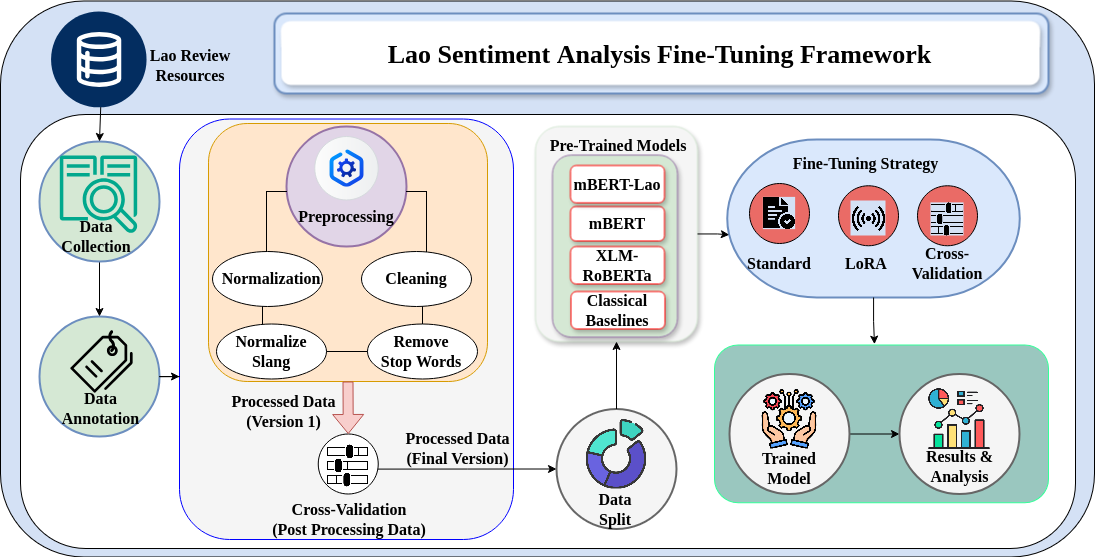
\includegraphics[width=\textwidth]{figures/Lao_Finetuning_Framework_Sentiment_Analysis.png}
\caption{Overall methodology framework for Lao sentiment classification, including dataset preparation, model selection, and training strategies.}
\label{fig:methodology_framework}
\end{figure}

Figure~\ref{fig:methodology_framework} summarizes the benchmark in three stages. The workflow begins with Google Play review collection, binary annotation, normalization, cleaning, and the post-processing audit used to construct the final split. It then trains XLM-RoBERTa, mBERT, mBERT-Lao, TextCNN, and TF-IDF baselines under the strategy variants applicable to each family, including Full Fine-tuning, LoRA, from-scratch training, and 3-fold cross-validation. Finally, the pipeline exports checkpoints, validation predictions, standard metrics, timing summaries, and false-positive/false-negative artifacts for the later analysis sections.

\subsection{Training Objective}
\label{subsec:training_objective}

PLM runs minimize weighted cross-entropy loss. Class weights compensate for the moderate label imbalance in the final dataset. For a training set of $N$ samples and two sentiment classes, the objective is
\begin{equation}
\mathcal{L} = - \sum_{i=1}^{N}\sum_{c=1}^{2} w_c y_{i,c}\log \hat{y}_{i,c},
\label{eq:loss}
\end{equation}
where $w_c$ is the weight for class $c$, $y_{i,c}$ is the one-hot target, and $\hat{y}_{i,c}$ is the predicted probability for class $c$.

We train the PLMs with standard pretrained-model tooling and fine-tuning practice \cite{han2021pre,min2023recent}, using a learning rate of $1e^{-5}$, weight decay 0.01, warmup ratio 0.1, and maximum sequence length 128. For Full Fine-tuning and LoRA, the best checkpoint is selected by validation loss. TextCNN uses the same epoch budget, batch sizes, and sequence length, but it initializes all parameters from scratch. The classical baselines use the same split and train TF-IDF character $n$-gram features from 3 to 5 with \texttt{min\_df}=2 and at most 50,000 features before classifier fitting.

Algorithm~\ref{alg:benchmark_pipeline} summarizes the unified benchmark pipeline used throughout the experiments. It reflects the fixed-split baseline runs, the PLM-based fixed-split runs, and the separate 3-fold cross-validation setting reported later in Section~\ref{sec:experiments}.

\begin{algorithm}[H]
\caption{Unified training and evaluation pipeline for Lao sentiment classification}
\label{alg:benchmark_pipeline}
\small
\begin{algorithmic}[1]
\Require fixed-split training set $D_{\text{train}}$, validation set $D_{\text{val}}$, PLM set $\mathcal{M}$, baseline set $\mathcal{B}$, strategies $\mathcal{S}=\{\text{FT},\text{LoRA}\}$
\Ensure prediction files, metrics, timing statistics, and error-analysis artifacts
\ForAll{$b \in \mathcal{B}$}
    \State compute TF-IDF features $\Phi(x)$ for $x \in D_{\text{train}}$
    \State $\psi_b \leftarrow \arg\min_{\psi} \mathcal{L}_{\text{train}}(\psi, \Phi(D_{\text{train}}))$
    \State $\hat{y} \leftarrow f_{\psi_b}(\Phi(x))$ for $x \in D_{\text{val}}$, evaluate metrics
\EndFor
\ForAll{$m \in \mathcal{M}$}
    \ForAll{$s \in \mathcal{S}$}
        \State load tokenizer and pretrained checkpoint for $m$
        \If{$s=\text{LoRA}$}
            \State inject LoRA adapters $BA$ via Eq.~\eqref{eq:lora_opt}
        \Else
            \State enable end-to-end updates via Eq.~\eqref{eq:full_ft}
        \EndIf
        \State minimize $\mathcal{L}$ on $D_{\text{train}}$ via Eq.~\eqref{eq:loss}
        \State $\psi^* = \arg\min_{\psi} \mathcal{L}(\psi, D_{\text{val}})$
        \State compute $\hat{y} = f_{\psi^*}(x)$ for $x \in D_{\text{val}}$, store metrics
    \EndFor
    \For{$k=1$ to $3$}
        \State partition $D_{\text{train}} \rightarrow \{ D_{\text{train}}^{(k)}, D_{\text{val}}^{(k)} \}$
        \State $\psi^{(k)} \leftarrow \text{optimize}(\mathcal{L}, D_{\text{train}}^{(k)}, m)$
        \State $\hat{D}_{\text{val}}^{(k)} \leftarrow \{f_{\psi^{(k)}}(x) \mid x \in D_{\text{val}}^{(k)}\}$
    \EndFor
    \State compute $\text{Score}_{\text{CV}}$ using Eq.~\eqref{eq:score_cv}
\EndFor
\State aggregate $\hat{D}_{\text{val}}$ and metrics to produce final artifacts
\end{algorithmic}
\end{algorithm}


\section{Experiments}
\label{sec:experiments}

This section outlines the experimental configuration, baseline selections, and evaluation metrics. We then present a comparative analysis of our findings regarding predictive performance, error patterns, and computational efficiency across the evaluated models.

\subsection{Experimental Setup}
\label{subsec:experimental_setup}

We begin by specifying the compared systems, the evaluation metrics, and the implementation details required to reproduce the benchmark.

\subsubsection{Compared Models}
The benchmark combines classical baselines, a lightweight neural baseline, and PLM-based models. The classical group contains Logistic Regression, SVM, and Decision Tree. The neural baseline is TextCNN, evaluated under From-Scratch training and 3-Fold Cross-Validation. The PLM group contains XLM-RoBERTa, mBERT, and mBERT-Lao, each evaluated with Full Fine-tuning, LoRA, and 3-Fold Cross-Validation. This setup creates a controlled comparison between sparse models, a compact neural model, and pretrained transformers on the same Lao review data.

The classical baselines were trained on the same fixed train-validation split used for the fixed-split PLM runs. They use character-level TF-IDF features with an $n$-gram range of 3-5, \texttt{min\_df}=2, and at most 50,000 features. Logistic Regression and SVM were implemented through \texttt{SGDClassifier} with \texttt{log\_loss} and \texttt{hinge} objectives, respectively, while Decision Tree used \texttt{max\_depth}=40 and \texttt{min\_samples\_leaf}=2. TextCNN uses 128-dimensional trainable embeddings, 128 filters for each kernel size in $\{3,4,5\}$, and dropout 0.3, giving the benchmark a compact neural reference that does not depend on pretrained weights.

\subsubsection{Evaluation Metrics}
We report Accuracy, Precision-macro, Recall-macro, and F1-macro, which are standard evaluation measures for text classification and information retrieval tasks \cite{opitz2024closer,tan2023survey}. Because the dataset is moderately imbalanced, F1-macro is treated as the main comparison metric, while the remaining metrics are used to show overall correctness and class-level balance.

For binary sentiment classification, Accuracy is defined as
\begin{equation}
\mathrm{Accuracy} = \frac{TP + TN}{TP + TN + FP + FN}.
\end{equation}
For each class $c \in \{0,1\}$, let
\begin{equation}
P_c = \frac{TP_c}{TP_c + FP_c}, \qquad R_c = \frac{TP_c}{TP_c + FN_c}.
\end{equation}
The macro-averaged scores reported in this paper are then
\begin{equation}
\mathrm{Precision}_{\mathrm{macro}} = \frac{1}{C}\sum_{c=1}^{C} P_c,\quad
\mathrm{Recall}_{\mathrm{macro}} = \frac{1}{C}\sum_{c=1}^{C} R_c,\quad
\mathrm{F1}_{\mathrm{macro}} = \frac{1}{C}\sum_{c=1}^{C} \frac{2P_cR_c}{P_c + R_c},
\end{equation}
where $c$ indexes a sentiment class and $C=2$ for the negative and positive labels. Here, $TP$, $TN$, $FP$, and $FN$ denote true positives, true negatives, false positives, and false negatives, respectively, while $TP_c$, $FP_c$, and $FN_c$ are the corresponding class-specific counts used to compute $P_c$ and $R_c$ for class $c$.

\subsubsection{Implementation Details}
The experiments use the final filtered Lao review dataset described in Section~\ref{subsec:dataset_statistics}. Logistic Regression, SVM, Decision Tree, and fixed-split TextCNN were trained on the same validation split as the fixed-split PLM runs, while 3-fold cross-validation was applied on the training partition for the PLMs and for TextCNN. The exact hyperparameters are listed in Table~\ref{tab:training_config}; the main difference across PLM runs is whether the full backbone is updated or only LoRA adapters are trained.

\begin{table}[H]
\centering
\caption{Training configuration used in the experiments.}
\small
\begin{tabular}{@{}ll@{}}
\toprule
\textbf{Component} & \textbf{Configuration} \\
\midrule
PLM epochs & 25 \\
Batch size / eval batch size & 16 / 32 \\
Maximum sequence length & 128 \\
Learning rate & $1 \times 10^{-5}$ \\
Weight decay & 0.01 \\
Warmup ratio & 0.1 \\
Cross-validation & Stratified $K=3$ \\
LoRA setting & $r=16$, $\alpha=32$, dropout $=0.1$ \\
TextCNN setting & Embedding 128, filters 128, kernels 3/4/5, dropout 0.3 \\
Best-model criterion & Validation loss \\
Baseline features & TF-IDF char $n$-grams (3-5), max 50,000 \\
\bottomrule
\end{tabular}
\label{tab:training_config}
\end{table}

\begin{table}[H]
\centering
\caption{Runtime environment recorded in the experiment artifacts.}
\small
\begin{tabular}{@{}ll@{}}
\toprule
\textbf{Hardware item} & \textbf{Recorded value} \\
\midrule
CPU & 1 physical core / 2 total cores \\
RAM & 12.67 GB \\
GPU & Tesla T4 \\
GPU memory & 14.56 GB \\
Recorded hardware scope & 14 experiment folders \\
\bottomrule
\end{tabular}
\label{tab:hardware_env}
\end{table}

\subsection{Results and Discussion}
\label{subsec:results_discussion}

We now examine the main performance pattern and use error and efficiency analyses to explain the observed trade-offs.

\subsubsection{Overall Performance}
Taken together, Table~\ref{tab:overall_results} and Figure~\ref{fig:metric_overview} indicate that backbone suitability matters more than simply moving from sparse to neural baselines, or from LoRA to Full Fine-tuning within the same PLM family. TextCNN provides a strong middle point: on the fixed split it outperforms Logistic Regression and approaches SVM, yet the best scores still come from the XLM-RoBERTa variants. This interpretation is consistent with low-resource sentiment studies that attribute transfer quality mainly to language fit and data characteristics rather than to simply updating more parameters \cite{lamin2025cross,subramanian2025kec_tech_titans,chowdhury2025mysticciol}. The benchmark also shows that sparse baselines remain meaningful for Lao app reviews, suggesting that the task still contains strong lexical sentiment cues even when pretrained encoders are available.

\begin{table}[H]
\centering
\caption{Overall performance grouped by model family and training strategy.}
\small
\renewcommand{\arraystretch}{1.2}
\setlength{\tabcolsep}{6pt}

\begin{tabular}{|p{0.22\textwidth}|p{0.22\textwidth}|
S[table-format=1.4]|
S[table-format=1.4]|
S[table-format=1.4]|
S[table-format=1.4]|}

\hline
\textbf{Model Family} & \textbf{Training Strategy} & \textbf{Acc.} & \textbf{F1} & \textbf{Prec.} & \textbf{Rec.} \\
\hline

{\textbf{XLM-RoBERTa}}
& Full Fine-tuning & {\bfseries 0.9664} & {\bfseries 0.9617} & {\bfseries 0.9544} & {\bfseries 0.9702} \\
\cline{2-6}
& LoRA & 0.9642 & 0.9589 & 0.9539 & 0.9645 \\
\cline{2-6}
& Cross-Validation & 0.9648 & 0.9597 & 0.9541 & 0.9659 \\
\hline

{\textbf{mBERT}}
& Full Fine-tuning & 0.6969 & 0.6057 & 0.6336 & 0.6012 \\
\cline{2-6}
& LoRA & 0.6901 & 0.6048 & 0.6253 & 0.6004 \\
\cline{2-6}
& Cross-Validation & 0.6967 & 0.6137 & 0.6350 & 0.6084 \\
\hline

{\textbf{mBERT-Lao}}
& Full Fine-tuning & 0.9407 & 0.9328 & 0.9241 & 0.9437 \\
\cline{2-6}
& LoRA & 0.9326 & 0.9235 & 0.9154 & 0.9335 \\
\cline{2-6}
& Cross-Validation & 0.9375 & 0.9285 & 0.9228 & 0.9350 \\
\hline

{\textbf{TextCNN}}
& From Scratch & 0.9477 & 0.9403 & 0.9338 & 0.9478 \\
\cline{2-6}
& Cross-Validation & 0.9339 & 0.9242 & 0.9192 & 0.9298 \\
\hline

{\textbf{Classical baselines}}
& Logistic Regression & 0.9451 & 0.9370 & 0.9322 & 0.9425 \\
\cline{2-6}
& SVM & 0.9505 & 0.9436 & 0.9363 & 0.9522 \\
\cline{2-6}
& Decision Tree & 0.8878 & 0.8721 & 0.8662 & 0.8792 \\
\hline

\end{tabular}

\label{tab:overall_results}
\end{table}

\begin{figure}[H]
\centering
\includesvg[width=\textwidth]{figures/lineplot_metrics}
\caption{Metric comparison across all benchmarked settings, sorted by F1-macro.}
\label{fig:metric_overview}
\end{figure}

\subsubsection{Domain Adaptation Analysis}
The gap between mBERT-Lao and generic mBERT suggests that Lao support is not a minor implementation detail but a substantive source of performance difference. This interpretation aligns with LaoPLM and related low-resource work, which argue that multilingual pretraining can under-serve Lao when tokenization behavior and corpus coverage are mismatched \cite{lin2022laoplm,lamin2025cross}. TextCNN further shows that a compact neural model can learn useful review-local patterns from scratch, but its lower cross-validation score suggests that it is more sensitive to split variation than the strongest pretrained models. At the same time, the competitiveness of SVM and Logistic Regression indicates that many app-review decisions are driven by local lexical cues and short formulaic complaints. In other words, domain adaptation in this dataset appears to depend on both language-aware representations and sensitivity to concise, review-specific expressions.

\subsubsection{Error Analysis}
Figure~\ref{fig:error_analysis} helps explain why the model ranking separates so clearly. The strongest systems maintain a more balanced error profile, whereas weaker multilingual transfer is associated with a clear positive-class bias. This matters because the difficult cases are not random; they are concentrated in short complaint-like comments, code-mixed fragments, and mixed-polarity reviews that combine a problem report with a request, update, or partially positive tone. Related low-resource sentiment studies likewise report that short, informal, and mixed-language comments are a recurring source of ambiguity \cite{subramanian2025kec_tech_titans,chowdhury2025mysticciol}, but the present results suggest that these cases are especially consequential for Lao app reviews, where limited context and informal phrasing amplify ambiguity.

\begin{figure}[H]
\centering
\includesvg[width=\textwidth]{figures/error_analysis_overview}
\caption{Error-analysis overview based on the aggregated false-positive and false-negative samples from all experiments. Panel (a) reports raw false-negative and false-positive counts, while panel (b) shows the corresponding error composition percentages for the same experiments.}
\label{fig:error_analysis}
\end{figure}

Table~\ref{tab:error_examples} illustrates this pattern qualitatively. False positives are usually short complaints whose negative intent is expressed indirectly or through code-mixed wording, whereas false negatives more often contain softened criticism, requests, or mixed cues. The dominant failure mode is therefore semantic ambiguity in short feedback, rather than annotation instability alone.

\begin{table}[H]
\centering
\caption{Representative Examples of Fixed-Split Error Patterns}
\label{tab:error_examples}

\vspace{0.5em}

\footnotesize
\setlength{\tabcolsep}{5pt}
\renewcommand{\arraystretch}{1.25}

\begin{tabularx}{\textwidth}{
>{\hsize=0.95\hsize\raggedright\arraybackslash}X
>{\centering\arraybackslash}m{0.08\textwidth}
>{\hsize=1.05\hsize\raggedright\arraybackslash}X
>{\centering\arraybackslash}m{0.08\textwidth}
}

\toprule

\multicolumn{2}{c}{\textbf{False Positive}} &
\multicolumn{2}{c}{\textbf{False Negative}} \\

\cmidrule(r){1-2}
\cmidrule(l){3-4}

\textbf{Example} &
\textbf{Label} &
\textbf{Example} &
\textbf{Label} \\

\midrule

{\tablelaofont ບໍ} ok
{\scriptsize\textit{not OK}}
&
0
&
{\tablelaofont ເປັນຍັງຄື ທັງຫມົດທີ່ຈຫຼີ້ນບໍ່ໄດ້}

{\scriptsize\textit{why does nothing work?}}
&
1 \\

{\tablelaofont ປ່ຽນໂທລະສັບໃຫມ່}

{\scriptsize\textit{changed to a new phone}}
&
0
&
{\tablelaofont ຄັກຢູ່ ແຕ່ໃຫ້ອັບເດດດຸໂພດ}

{\scriptsize\textit{it is good, but please update it}}
&
1 \\

{\tablelaofont ເບີລະຫັດ} whatsapp

{\scriptsize\textit{WhatsApp verification code}}
&
0
&
{\tablelaofont ແຕ່ໃຫ້ປັບປຸງໃຫ້ໄວກ່ວาເກົ່າ}

{\scriptsize\textit{please make it faster}}
&
1 \\

bug {\tablelaofont ຫລາຍ}

{\scriptsize\textit{too many bugs}}
&
0
&
{\tablelaofont ໂຄ້ດດີ ຖ້າບໍ່ອັບເດດແອປ ແຮງຊິດີ}

{\scriptsize\textit{the code is good, but the update hurts the app}}
&
1 \\

{\tablelaofont ແອັບຊ່າສຸດ}

{\scriptsize\textit{the app is very slow}}
&
0
&
{\tablelaofont ຂອບເຂດສົ່ງ ກ້ວາງໄກລ ສົ່ງໄວ ບໍ່ມີບັນຫາ}

{\scriptsize\textit{wide service area, fast delivery, no problems}}
&
1 \\

\bottomrule

\end{tabularx}
\end{table}

Figure~\ref{fig:short_fail_wordcloud} provides a complementary phrase-level view of the same error set using the 30 most frequent short false-positive and false-negative samples. This visualization is intended as a qualitative summary of recurring failure expressions rather than as a replacement for the quantitative counts in Figure~\ref{fig:error_analysis}.

\begin{figure}[H]
\centering
\begin{minipage}[t]{0.48\textwidth}
\centering
\includesvg[width=\linewidth]{figures/short_fail_wordcloud_fp}

\vspace{0.25em}
{\small (a) False Positives}
\end{minipage}\hfill
\begin{minipage}[t]{0.48\textwidth}
\centering
\includesvg[width=\linewidth]{figures/short_fail_wordcloud_fn}

\vspace{0.25em}
{\small (b) False Negatives}
\end{minipage}
\caption{Phrase-level word clouds built from the 30 most frequent short false-positive and false-negative samples in the fixed-split experiments. Larger phrases indicate more frequently repeated failure cases.}
\label{fig:short_fail_wordcloud}
\end{figure}

\subsubsection{Practical Implications}
From a deployment perspective, the results support a tiered selection strategy. When predictive quality is the main priority, XLM-RoBERTa is the most reliable choice. When computational efficiency matters but a neural model is still preferred, TextCNN offers a useful middle ground: it reaches 0.9403 F1-macro on the fixed split while training in only 11.28 minutes. Within the PLM family, LoRA offers a better trade-off than retraining the full model. Although this study does not report dedicated inference latency, the much smaller trainable footprint of LoRA suggests lower adaptation and deployment overhead than full fine-tuning in resource-constrained settings. When infrastructure or maintenance constraints dominate, SVM remains a credible baseline because it is stable, interpretable, and inexpensive to train. More broadly, the benchmark suggests that practical Lao sentiment systems should be selected not only by raw accuracy, but also by how well they balance language fit, efficiency, and operational simplicity.

\begin{table}[H]
\centering
\caption{Efficiency comparison between Full Fine-tuning and LoRA.}
\resizebox{\textwidth}{!}{%
\begin{tabular}{|l|l|r|r|r|r|r|}
\hline
\textbf{Model} & \textbf{Strategy} & \textbf{Trainable params} & \textbf{Trainable ratio} & \textbf{Avg. epoch time (s)} & \textbf{Total train time (s)} & \textbf{F1-macro} \\
\hline
XLM-RoBERTa & Full Fine-tuning & 278,045,186 & 1.0000 & 267.31 & 6682.66 & 0.9617 \\
XLM-RoBERTa & LoRA & 1,476,866 & 0.0053 & 117.80 & 2945.07 & 0.9589 \\
mBERT & Full Fine-tuning & 177,854,978 & 1.0000 & 205.82 & 5145.48 & 0.6057 \\
mBERT & LoRA & 886,274 & 0.0050 & 116.92 & 2922.95 & 0.6048 \\
mBERT-Lao & Full Fine-tuning & 124,647,170 & 1.0000 & 177.52 & 4438.10 & 0.9328 \\
mBERT-Lao & LoRA & 1,476,866 & 0.0117 & 113.74 & 2843.53 & 0.9235 \\
\hline
\end{tabular}}
\label{tab:efficiency}
\end{table}

\begin{figure}[H]
\centering
\includesvg[width=\textwidth]{figures/lineplot_timing}
\caption{Timing comparison across all benchmarked settings, sorted by average epoch time.}
\label{fig:timing}
\end{figure}


\section{Conclusion}
\label{sec:conclusion}

In this study, we established a comprehensive benchmark for Lao sentiment classification, utilizing a large-scale, filtered dataset of real-world mobile application reviews. Our systematic evaluation of classical baselines, a lightweight TextCNN neural baseline, and advanced Pre-trained Language Models reveals that XLM-RoBERTa delivers the most robust performance, while Lao-specific pretraining significantly enhances cross-lingual transfer in under-resourced settings. Furthermore, we demonstrated that Parameter-Efficient Fine-Tuning (PEFT) via LoRA achieves a practical balance between predictive quality and computational efficiency, making it a viable strategy for resource-constrained deployments. TextCNN also emerges as a strong middle-ground option, outperforming Logistic Regression on the fixed split while training much faster than the PLMs. The persistent competitiveness of traditional SVM baselines further underscores the importance of localized lexical features in short, informal Lao feedback.

Despite these advancements, the study identifies critical challenges posed by linguistic ambiguity, noise, and semantic shifts in code-mixed environments. Future research should prioritize enhancing dataset diversity and label consistency, while exploring more granular analysis frameworks, such as aspect-level sentiment classification, to provide deeper insights into user experience. By releasing our dataset and trained models, we aim to support the development of more scalable and accurate NLP tools for the Lao digital ecosystem.

\bibliographystyle{IEEEtran}
\bibliography{references}

\end{document}
